\documentclass[conference]{IEEEtran}
\IEEEoverridecommandlockouts
% The preceding line is only needed to identify funding in the first footnote. If that is unneeded, please comment it out.
\usepackage{cite}
\usepackage{amsmath,amssymb,amsfonts}
\usepackage{algorithmic}
\usepackage{graphicx}
\usepackage{textcomp}
\usepackage{xcolor}
\usepackage{listings}

\def\BibTeX{{\rm B\kern-.05em{\sc i\kern-.025em b}\kern-.08em
    T\kern-.1667em\lower.7ex\hbox{E}\kern-.125emX}}
\begin{document}

\title{CENG435 Term Project-1 Report\\
{\footnotesize}
}

\author{\IEEEauthorblockN{Name Surname : Omer CETIN}
\IEEEauthorblockA{Student ID : 2257541 \\
}
\and
\IEEEauthorblockN{Name Surname : Oguzcan BUDUMLU}
\IEEEauthorblockA{Student ID : 2098820
}
}

\maketitle

\section{Introduction}
Before we started to do this homework, we wanted to get familiar with the GENI environment. So, we first did the lab0 assignment that was shared with us on METU Class. After completing the lab0, we were ready to start the homework. Then, we start to write scripts for each node on the topology one by one. We chose to write scripts in Python because of the convenience of Python for socket programming. Firstly scripts for the source and the broker were written then for routers and lastly, a script for the destination is written. We proceeded with testing the results of each node and analyzing how they behave according to our code. In the destination, we had to handle the data coming from the routers, because the destination has a responsibility of catching the data from both routers without missing them(in this case I refer to the destination dealing with another task of the node while there is data to catch, not the reliability of the protocol used), so to overcome this issue, we benefited threads. In the meantime, we run this scripts on our local computer. After we believe that they are working properly, we took a slice on GENI, we transferred each script to the remote virtual machines according to our topology. By the way, each node on the topology corresponds to a remote virtual machine. Then we run the scripts on the virtual machines, we had some issues with synchronization. We did the experiments adding the 1 millisecond, 20 milliseconds and 60 milliseconds delays over the links. Lastly, we collected the experiments' results to write this report. 

\section{Understanding The Topology}
\begin{figure}[ht]
  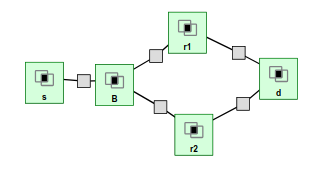
\includegraphics[width=\linewidth]{topology.png}
  \caption{Topology}
  \label{fig:boat1}
\end{figure}
In our topology, there are five nodes which have different roles in our network that we have built.\\
s node is the source that is simply the source of data and where the data is being sent over TCP to the broker.\\
B node is the broker which takes the data coming from the source node over TCP and forwards the data to the router 1 and router 2 over UDP. The broker also constantly listen to the source so that if the source sends any data, the broker will be able to catch them. The broker has a feature that is being able to receive the data over TCP and being able to send the data over UDP.\\
r1 and r2 are just simple routers which receive the data from the broker over UDP and forwards the data to the destination. The routers also listen to the broker if there is any data coming.\\
d is the destination where is the last stop of the data. The destination node constantly listens to the routers. In the destination, there is a thread run for each router. 

\section{Synchronization}
In order to calculate end-to-end delay, we needed to synchronize source and destination clocks. We used NTP (Network Time Protocol) by including the related library(ntplib) in the code for this purpose. We selected a server (one of the Google servers) so that round-trip time from both source node and destination node to this server is as close as possible so we made use of ping command to understand this closeness:
\begin{lstlisting}[language=bash]
  $ ping -c 100 time1.google.com |
  tail -1| awk '{print $4}' | 
  cut -d '/' -f 2
\end{lstlisting}

This command calculates average of 100 round-trip time between nodes. When we tried this in source and destination nodes, we saw their average 44.926 milliseconds and 44.897 milliseconds respectively. Since there is a tiny difference between them with respect to results in our experiments, we neglected them.

\section{Network Emulation}

On the virtual machines we executed the commands below to perform each experiment.\\
If we emulate delay in a virtual machine for the first time, the commands we need to execute are:\\
\\
In broker:
\begin{lstlisting}[language=bash]
  $ sudo tc qdisc add dev eth1 root 
  netem delay 1ms
  $ sudo tc qdisc add dev eth3 root 
  netem delay 1ms
\end{lstlisting}

In router 1:

\begin{lstlisting}[language=bash]
  $ sudo tc qdisc add dev eth2 root 
  netem delay 1ms
\end{lstlisting}


In router 2:

\begin{lstlisting}[language=bash]
  $ sudo tc qdisc add dev eth1 root 
  netem delay 1ms
\end{lstlisting}

After executing the commands above once, we continue by executing commands below:\\
\\
In broker:
\begin{lstlisting}[language=bash]
  $ sudo tc qdisc change dev eth1 root 
  netem delay 1ms 5ms distribution normal
  $ sudo tc qdisc change dev eth3 root 
  netem delay 1ms 5ms distribution normal
\end{lstlisting}

In router 1:

\begin{lstlisting}[language=bash]
  $ sudo tc qdisc change dev eth2 root 
  netem delay 1ms 5ms distribution normal

\end{lstlisting}


In router 2:

\begin{lstlisting}[language=bash]
  $ sudo tc qdisc change dev eth1 root 
  netem delay 1ms 5ms distribution normal

\end{lstlisting}

Note that commands above are written for the experiment of 1 milliseconds emulation delay with 5 milliseconds normal distribution. Other experiments can be performed by changing $1ms$ to $20ms$ or $60ms$.\\
Also note that interfaces (referred to eth1, eth2, eth3) are chosen with respect to the topology we are given.\\
\section{Experiment}
There are 3 experiments we have to do. In each experiment, we add a specific delay to the broker and routers with executing netem/tc commands on virtual machines. In the first experiment we add 1ms delay, in the second 20 milliseconds and in the third 60 milliseconds with 5 milliseconds normal distribution.
We have plotted the below graph according to results of the each experiment performed. \\
\begin{figure}[ht]
  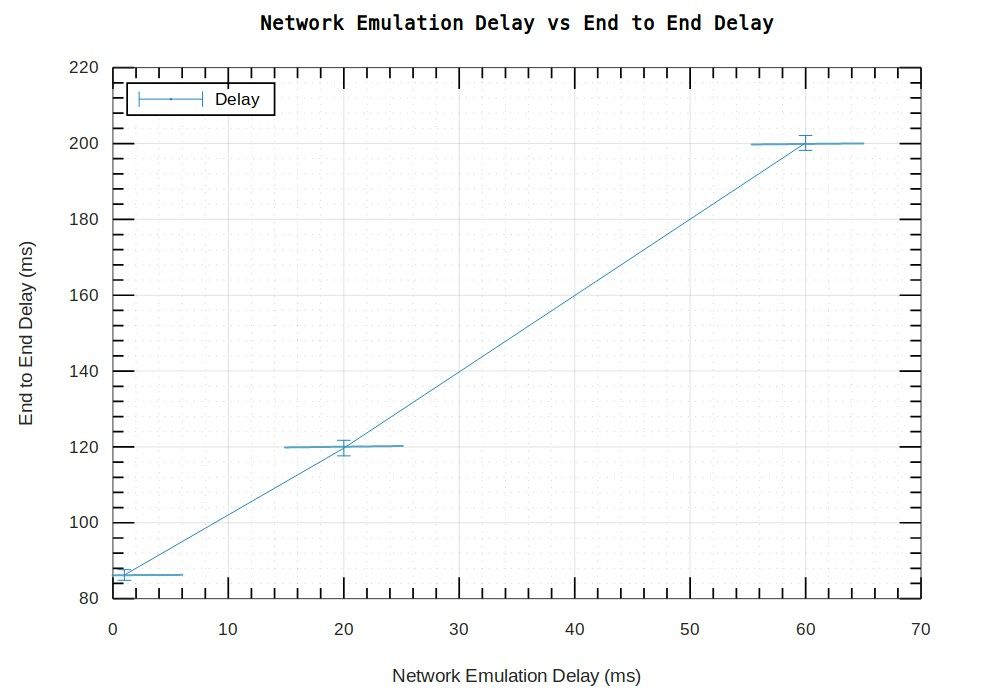
\includegraphics[width=\linewidth]{experiment.jpeg}
  \caption{Experiment}
  \label{fig:boat1}
\end{figure}\\
As shown in the graph above, when we change the network emulation delay, there is a change in end to end delay accordingly. The network emulation delay and end to end delay have almost a linear relationship.
We formed this graphic by using 50 samples i.e. sending 50 packets from source to destination.

We observed that end-to-end delay increases approximately twice as emulation delay we perform. For example, when we increase emulation delay from 0 to  20 milliseconds with 5 milliseconds normal distribution , end-to-end delay mean increased from 86.23 milliseconds to 119.69 milliseconds. For 20 milliseconds emulation delay, 33.46 milliseconds end-to-end delay existed. In a similar manner, when we increase emulation delay from 20 to  60 milliseconds with 5 milliseconds normal distribution, end-to-end delay mean increased from 119.69 milliseconds to 201.54 milliseconds. For 40 milliseconds emulation delay, 81.85 milliseconds end-to-end delay existed. We can see more clearly below:
\\
\\
\begin{tabular}{cc}
\textbf{Emulation Delay(ms)} & \textbf{End-to-End Delay(ms)} \\
1 +- 5                       & 86.23 +- 1.41                      \\
20 +- 5                      & 119.69 +- 2.06                     \\
60 +- 5                      & 201.54 +- 1.86                    
\end{tabular}
\\
\\
Since we emulate same amount of delays in both broker and routers, we see approximately doubled amount of emulation delay in our results.





\end{document}
